%\textit{Method and simulation framework development and implementation](https://github.com/laurieKell/mydas/wiki/3-Method-and-simulation-framework-development-and-implementation). A number of data-limited methods exist. In order to compare the performance of these methods it would be useful to implement them all in the same framework, e.g. R. New methods may also be developed in the same framework.}

A number of data-limited methods already exist, in order to compare their performance they need to be run in a common framework. Therefore methods were interfaced to R, using the Fishery Library in R (\textbf{FLR}) \citep{kell2007flr} a toolset that is composed of a variety of packages, covering the various steps in the fisheries advice and simulation workflow. Using \textbf{FLR} means that advantage can be taken of existing methods, and that dissemination and support is easier and will be maintained after the life of the project. 

To identify the appropriate advice given the quality of data rules ICES classifies stock assessments into six \href{http://www.ices.dk/sites/pub/Publication Reports/Advice/2015/2015/General_context_of_ICES_advice_2015.pdf}{categories} on the basis of the available data, e.g. total landings, indices of abundance, length frequency and age data. 

\begin{description}[rightmargin=\dimexpr\linewidth-15cm-\leftmargin\relax]
 \item[Category 1: stocks with quantitative assessments]  Full analytical assessments and forecasts as well as stocks with quantitative assessments based on production models.

\item[Category  2: stocks  with  analytical  assessments  that  are  only  treated  qualitatively] 
Quantitative assessments and forecasts which for a variety of reasons are considered indicative of trends in fishing mortality, recruitment, and biomass.

\item[Category 3: stocks for which survey based assessments indicate trends] 
Survey or other indices are available that provide reliable indications of trends in stock metrics, such as total mortality, recruitment, and biomass.

\item[Category 4: stocks for which only reliable catch data are available] 
Time series of catch can be used to approximate MSY.

\item[Category 5: landings only]
Only landings data are available.

\item[Category 6: negligible landings]
Landings are negligible in comparison to discards and stocks that are  primarily caught as bycatch species in other targeted fisheries 
\end{description}


For data limited stocks a number of methods already exist, for example the ICES Working Group on Category 3 and 4 stocks \href{ 
http://www.ices.dk/sites/pub/Publication Reports/Expert Group Report/acom/2017/WKMSYCAT34/01 WKMSYCAT34 REPORT 2017.pdf}{(WGMSYCAT34)} has been working on rules for survey-based assessments which indicate trends in stock status (Category 3) or for which only catch data are available (Category 4). 

Data limited methods in use worldwide were summarised in a \href{https://docs.google.com/spreadsheets/d/17_qQdzDY41ZrL0yT6QtHpUR4_ydxx_xfCh4GiDqYymU/edit?usp=sharing}{google spreadsheet}. Following which five catch and three length based methods, were then selected for simulation testing. The choice of methods was based on the availability of code, whether the method had been peer reviewed and the appropriateness of estimated quantities for use as proxy reference points. The methods were then simulation tested \citep{pons2019catchlen} in order to select the best catch and length-only methods.


\subsubsection*{Catch Only}

Catch-only assessment methods evaluated were Catch-Maximum Sustainable Yield \citep[Catch-MSY][]{martell2013simple}, Depletion Based  Stock Reduction Analysis \citep[DBSRA][]{dick2011depletion}, Simple Stock Synthesis \citep[SSS][]{cope2013implementing}, an extension of Catch-MSY (CMSY), and State Space Catch Only Method \citep[SSCOM][]{thorson2015catch}. Length based methods evaluated were Length Based Spawning Potential Ratio \citep[LBSPR][]{hordyk2014novel,hordyk2015evaluation}, Length-Based Integrated Mixed Effects \citep[LIME][]{rudd2017accounting}, and Length-Based Bayesian \citep[LBB][]{froese2018new}.

Catch-MSY  is based on stock reduction analysis (SRA) that assume a Schaefer biomass dynamic model. Inputs are a time series of removals, priors for the population rate of increase at low population size ($r$), carrying capacity ($K$), and a probability distribution of stock depletion in the first, final and (optionally) middle years. CMSY, extends Catch-MSY by using a Monte-Carlo filter to fix systematic biases in the Catch-MSY. 

DBSRA further modifies the SRA approach by using Monte Carlo draws from the parameter distributions for M, $F_{MSY}/M$, $B_{MSY}/B_0$, depletion, and age at maturity ($A_{mat}$) to separate total biomass into immature and mature biomass using a delay-difference production model. 

SSS is based on Stock Synthesis  \citep{methot2013stock}, and fixes all parameters in a Stock Synthesis model except for initial recruitment ($lnR_0$). An artificial index of abundance that represents the relative stock biomass is used for fitting where the first value of the index is 1, and the value in the final year represents depletion (i.e. the proportion of the population left in the final year). Values of steepness ($h$) and depletion are randomly drawn from a specified distribution using a Monte Carlo approach and $lnR_0$ is then estimated. 

State Space Catch Only Model (SSCOM) is a Bayesian state-space model that integrates across three stochastic functional forms, variation in effort, population dynamics and fishing efficiency \citep{thorson2013new}. Similar to the original Catch Only Model \citep{vasconcellos2005overview}, a coupled biomass-effort dynamics model is assumed. 

\subsubsection*{Length Only}


LBSPR, estimates the proportion of the unfished reproductive potential per recruit  (SPR) under a given level of fishing pressure. In an exploited population is calculated as a function of the ratio of fishing mortality to natural mortality ($F/M$), selectivity, and the two life-history ratios $M/k$ and $L_m/L_{\infty}$; where $k$ is the von Bertalanffy growth coefficient, $L_m$ is the size of maturity and $L_{\infty}$ is asymptotic size. The inputs are length at maturity specified in terms of $L_{50}$ and $L_{95}$ (the size at which 50\% and 95\% of a population matures) and length frequency data. LBSPR is an equilibrium based method and assumes asymptotic selectivity, von Bertalanffy growth, length at-age is normally distributed, rates of natural mortality are constant across adult age classes, recruitment is constant over time, and growth rates remain constant across the cohorts within a stock. 

LIME like LBSPR uses biological information and the length composition of the catch to estimate F and SPR. Unlike LBSPR, however, it does not assume equilibrium conditions and uses mixed effects to  estimate changes in recruitment and fishing mortality separately over time. 

LBB is a simple and fast method for estimating relative stock size that uses a Bayesian Monte Carlo Markov Chain (MCMC) approach. LBB uses pre-specified priors on parameters, and thus, technically does not require any inputs other than length frequency data. It does provides the user the option to specify priors for $L_{\infty}$, length at first capture ($L_c$), and relative natural mortality ($M/k$). $F/M$ is estimated over the age range represented in the length-frequency sample. 


\subsubsection*{Evaluation}

The methods were simulation tested for three life history types (short, medium and long-lived), three historical exploitation scenarios, and three depleted levels \citep{pons2019catchlen}. The results of the simulations are shown in Figure \ref{fig:cln}. Of the five catch based methods SSCOM performs poorly in terms of precision and bias, while SSS is the least biased and DBSRA the most precise. The length based methods tend to perform less well than the catch based methods, while LIME is the least biased while LBSPR is the most precise.

\begin{figure*}[h!]\centering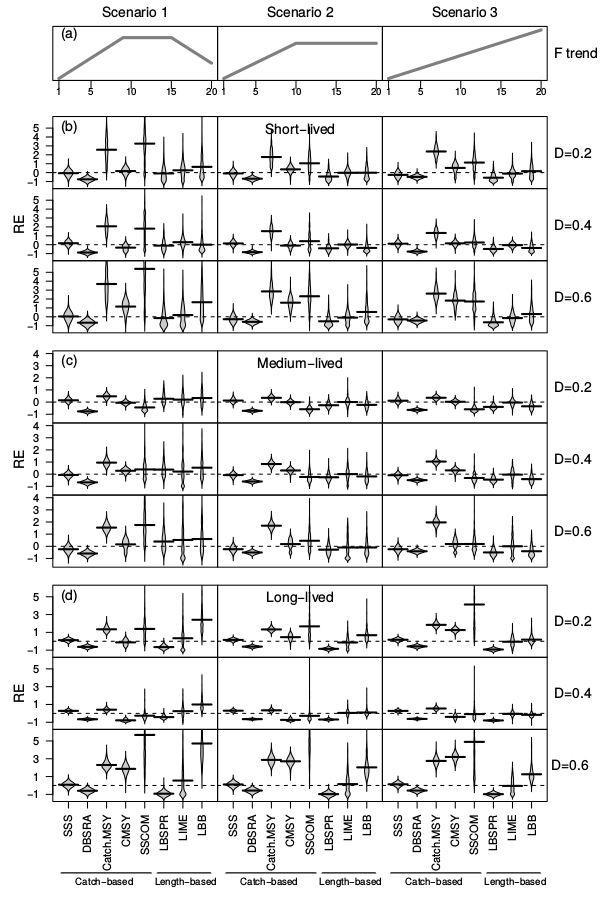
\includegraphics[width=6in]{figs/Figure_1.png}\label{fig:cln}\caption{Relative error (RE) in exploitation rate for all the catch-based and length-based models considered under the different harvest scenarios (a) and depletion scenarios for differing life histories, (b) short-lived, (c) medium-lived, and (d) long-lived.}
\end{figure*}

Bias and precision are both important factors to consider when assessing fish stocks. Bias reflects how close an estimate is to a known value; precision reflects reproducibility of the estimate. For example, if an assessment is to be re-conducted every year to monitor the impact of a management measure, a precise but biased method would be able to detect a trend better than an unbiased but imprecise method. Like all scientific instruments, this trade-off requires calibration to correct for the bias, and such calibration can be explored using closed-loop simulations (i.e. MSE), where the choice of parameters and reference points in a Management Procedure are tuned (i.e. calibrated) to meet the desired management objectives as represented by the Operating Model. Thus, a biased method (e.g., DBSRA) may be preferable to one that is less biased, but more imprecise (e.g., LIME). Alternatively, imprecision can be addressed through the choice of the percentile (e.g., median being the 50\% percentile value) for the derived model output used by management (e.g., catch or SPR); assuming that the true value is contained within the parameter distribution. For example, instead of taking the median value, one could instead use the derived model output associated with the 40th percentile to incorporate risk tolerance as reflected in the calculated imprecision. Such an approach \citep{Ralston2011meta} is used in fisheries management systems to directly incorporate scientific uncertainty (both bias and imprecision), and can also be explored and tuned using MSE.

The best performing catch-only methods were SSS and DBSRA, SSS was the least biased method while DBSRA was the most precise. A problem with SSS is that it is based on SS3 and so is a complicated method that requires a lot of assumptions in the form of fixed parameters. DBSRA in contrast is based on a biomass based stock production function and so requires fewer assumptions, it also allows data poor and data rich assessments to be compared, i.e. if an index of abundance could be developed then an ICES Category 3 assessment could be converted into a Category 1 assessment. This allows the value of information to be evaluated. Therefore DBSRA was selected for further evaluation.  

Both LBSPR and LIME use the same inputs, the main difference is that LIME is a non-equilibrium method, takes longer to run than LBSPR and often failed to converge, so although LIME estimates are less biased than LBSPR it is likely to perform poorly in closed loop simulations. LBB performed poorly in terms of both bias and precision. Therefore LBSPR was selected for the next stage of simulation evaluation.

